Uma outra pergunta seria: Como simular sistemas com dois pontos finais? Nesse caso pudemos retirar matrizes com entradas independentes porquê a distribuição era relacionada à $e^{\alpha H^2}$, mas agora teremos algo do tipo $e^{\alpha H^2 + H_0}$. Como fazer isso? Podemos tomar uma abordagem aproximada e checar por sua precisão posteriormente.

Queremos tirar autovalores de uma matriz $\tilde{X}$ tal que sua distribuição seja equivalente à dos movimentos brownianos independentes que não se cruzam com dois pontos finais. Note que de alguma forma, podemos tomar como base a matriz aleatória hermetiana de entradas gaussianas já discutida $X$. Isso nos dá a situação anterior. Mas ainda mais queremos manter o começo parecido mas fazer que, no final, os autovalores estejam separados em dois núcleos. Como os autovalores de uma matriz $X_o^2 = UVU^*$ tal que

\[ V = 
\begin{vmatrix}
	\lambda_1 & 0 & \cdots & \cdots & 0 \\
	0 & \lambda_1 &  &  & \vdots \\
	\vdots &  & \ddots &  & \vdots \\
	\vdots &  &  & \lambda_2 & 0 \\
	0 & \cdots & \cdots & 0 & \lambda_2
\end{vmatrix}
\]

Dessa forma se fizermos a composição dos dois terbos com uma função linear em $t$, teremos:

\[
X + f(t) UVU^*
\]

Que vai nos atender no sentido em que, quando $f(t) = 0$, em $t=0$ o comportamento é dominado pelo primeiro termo. Enquanto isso, quando a variância volta a diminuir nas entradas de $X$, o segundo termo domina, e, no final, dita as posições das partículas. Podemos testar nosso método. Implementemos:


\inputminted[
frame=lines,
framesep=2mm,
baselinestretch=1.2,
bgcolor=white,
fontsize=\footnotesize,
linenos
]{Python}{code/BrownianMultFinal.py}


E teremos algo do tipo:

\begin{center}
	\includegraphics[scale=0.9]{images/nonintersectBrownianPart-2f}
\end{center}


\subsection{Tracy Widom}

Uma das formas de validar nossa simulação é aproveitando de um resultado conhecido para esta distribuição. Tomamos $\gamma = \gamma(t) = \mathbb{E}[\lambda_{max}]$. Se definirmos a distribuição na borda para uma matriz de tamanho $N$ quando $N \rightarrow \infty$, veremos que

\[
\frac{\lambda_max - \mathbb{E}[\lambda_{max}]}{N^{\alpha}}
\]

Deve ser a densidade da distribuição quando $\alpha = -\frac{2}{3}$ para toda a extensão externa da distribuição. Essa distribuição se nomeia Tracy Widom e tem formato bem conhecido. Note que se o expoente não for compatível com a distribuição observada, ele deve, no limite fazer com que ela se torne 'singular' em algum sentido, esmague ela no eixo em $x$ ou $y$. Logo, idealmente, usaríamos matrizes extremamente grandes. O problema de autovalores, contudo, é complexo e leva tempo para tais matrizes. Faremos um compromisso e tentaremos observar a diferenciação da distribuição real.

Primeiro, a média. Faremos isso numericamente. Queremos algo do tipo,

 \begin{center} 	\includegraphics[scale=0.9]{images/nonintersectBrownianPart-M2-coutour}
 \end{center}
 
Para simplicar o gasto temporal calculemos para um passo específico múltiplos experimentos, uma vez que sabemos calcular a matriz que dá sua distribuição.

\inputminted[
frame=lines,
framesep=2mm,
baselinestretch=1.2,
bgcolor=white,
fontsize=\footnotesize,
linenos
]{Python}{code/TracyWidow.py}

Com $N=1000$, para o momento $t=0.5$ calculamos múltiplas iterações

\begin{center} 	\includegraphics[scale=0.9]{images/nonintersectBrownianPart-M2-t}
\end{center}

Agora podemos plotar o histograma para os extremos. Especificamente para o extremo superior:


\begin{center} 	\includegraphics[scale=0.7]{images/nonintersectBrownianPart-tracywidow05}
\end{center}


Algo está estranho. Parece que o histograma está mais espalhado do que o esperado. O que pode estar ocorrendo? Vemos nos dados que a variação está de acordo com o histograma. Os dados variam em média algo na ordem de $\pm 1$. Escalado por $N^{\frac{2}{3}}$, dá o resultado observado. De alguma forma os dados parecem com o 'formato' correto, até sua assimetria pode ser observada. E os dados parecem simetrizados para o autovalor máximo e mínimo. Uma suspeita é que alguma escala que dependa de $\sigma$ deve ser aplicada, isso se dá principalmente pela pergunta: Isso se repete em outros momentos da simulação? Que tem ilustrada resposta:

\begin{center} 	\includegraphics[scale=0.7]{images/nonintersectBrownianPart-tracywidow001}
\end{center}

Isso se repetiria para o caso de borda de um único final? Se calcularmos como usualmente as Pontes de Dyson para um único ponto final, veremos a distribuição de Tracy-Widom? Isso indicaria um erro, não na escala, mas no nosso modelo (Principalmente porque os modelos de aproximam quando $t \rightarrow 0$). Para este, teríamos em $t=0.5$:

\begin{center} 	\includegraphics[scale=0.7]{images/nonintersectBrownianPart-tracywidow-1-05}
\end{center}

Que parece precisar da mesma escala que o caso anterior. De qual escala estamos falando? Note a expressão

\[
	N^{\frac{2}{3}} \left( \frac{\lambda_{max} - 2\sigma\sqrt{N}}{\sigma \sqrt{N}}  \right) 
\]

Algo assim parece mais razoável. O $\lambda$ médio depende de $\sigma$ e $N$. Enquanto $\sigma \sqrt{N}$ escala com dependência das mesmas variáveis, que parecem ser importantes. Com essa nova distribuição podemos refazer a distribuição para $t=0.5$,

\begin{center} 	\includegraphics[scale=0.7]{images/nonintersectBrownianPart-tracywidow05-distreal}
\end{center}

e para $t=0.01$,

\begin{center} 	\includegraphics[scale=0.7]{images/nonintersectBrownianPart-tracywidow001-distreal}
\end{center}

A média ainda poderia ser dada por experimento desde que se centralize a distribuição também.

De fato isso também vale para todo o contorno com exceção do ponto de bifurcação interno, onde gostaríamos de ver $\alpha=-\frac{3}{4}$. Ou seja,

\[
N^{\frac{3}{4}} \left( \frac{\lambda_{max} - 2\sigma\sqrt{N}}{\sigma \sqrt{N}}  \right) 
\]

Para nosso caso de uma matriz $1000\cdot 1000$ procuremos $t$ apropriado para a distribuição dos autovalores médios. Note os autovalores para múltiplos experimentos:


\begin{center} 	\includegraphics[scale=0.7]{images/nonintersectBrownianPart-tracywidow-central_tmais}
\end{center}

\begin{center} 	\includegraphics[scale=0.7]{images/nonintersectBrownianPart-tracywidow-central_tmenos}
\end{center}

Para $t=0.9840$ então, faremos para os autovalores médios:

\begin{center} 	\includegraphics[scale=0.7]{images/nonintersectBrownianPart-tracywidow-central}
\end{center}

E de fato, se utilizarmos $\alpha = \frac{2}{3}$,

\begin{center} 	\includegraphics[scale=0.7]{images/nonintersectBrownianPart-tracywidow-central-23}
\end{center}


\subsection{O diamante Asteca}

\subsubsection{O tabuleiro de xadrez}

Outros modelos estocásticos mantém de alguma forma a universalidade que aparece na distribuição de autovalores. Antes, uma introdução.

Se quisermos fazer o tiling de um tabuleiro de xadrez com dominós de $2x1$, sabemos que isso é possível, inclusive por tilings triviais.

\begin{center}
	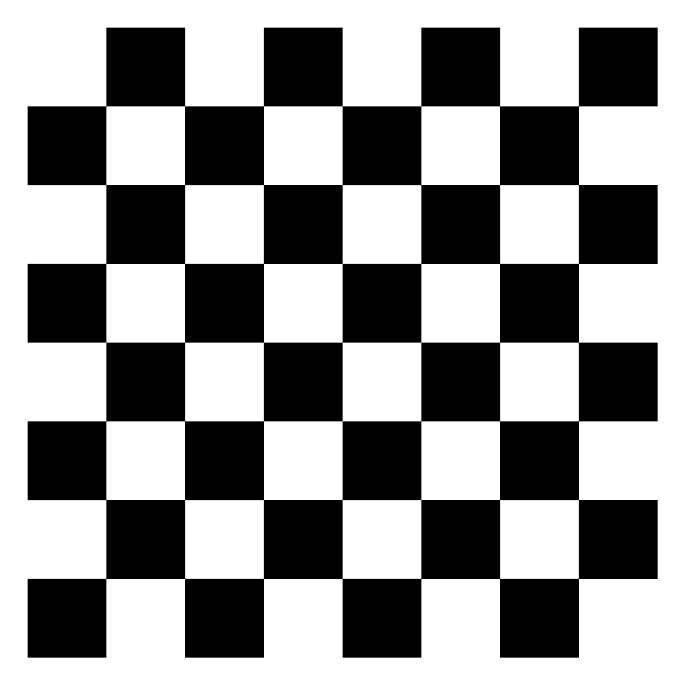
\begin{tikzpicture}[x=1cm]
		\foreach \y in {0,2,...,6}{
			\foreach \x in {0,2,...,6}{
				\fill (\x,\y) rectangle (1+\x,1+\y) rectangle (2+\x,2+\y);}}
	\end{tikzpicture}
\end{center}

Com tilings que podemos fazer trivialmente:

\begin{center}
	
\begin{tikzpicture}[x=1cm]
		\foreach \y in {0,1,...,6}{
			\foreach \x in {0,2,...,6}{
				\draw (\x,\y) rectangle (1.9+\x,0.9+\y) rectangle (2+\x,0.9+\y);}}
	\end{tikzpicture}
\end{center}

Um interessante detalhe é demonstrar se é possível fazer o mesmo retirando uma peça do tabuleiro. A demonstração é razoavelmente trivial e nos mostra que é impossível fazer tal coisa. Basta notar que todas peças do dominó devem ocupar uma peça branca e uma peça preta. De tal forma que, retirando uma peça, tal cobrimento não pode ser possível pois restará um número ímpar de alguma classe. 

É sempre possível fazer o tiling de um tabuleiro onde se retire duas peças arbitrárias? Claro, se elas forem de mesma cor, a mesma demonstração anterior vale e não será possível fazer o cobrimento. Mas e se forem cores complementares? A demonstração nos diz que é possível retirando pares de cores. Como? É possível mostrar que é pode-se definir um contorno que sigam as células do tabuleiro. Ou seja, um caminho em loop no tabuleiro de peças alternadas que pode ser preenchido por dominós em sequência. Retiradas duas peças do caminho, temos dois casos, um degenerado quando se retira peças sequenciais e é trivial que pode-se preencher o resto (equivalente a retirar um dominó do caminho completo) ou separa-se e duas fitas independentes. Neste caso, basta notar que ambas fitas devem ter um quantidade par de casas alternadas e seguirá trivialmente que é possível as preencher.

\subsubsection{De quantas formas preenchemos?}

Imagine uma forma qualquer sem buracos.

\begin{center}
	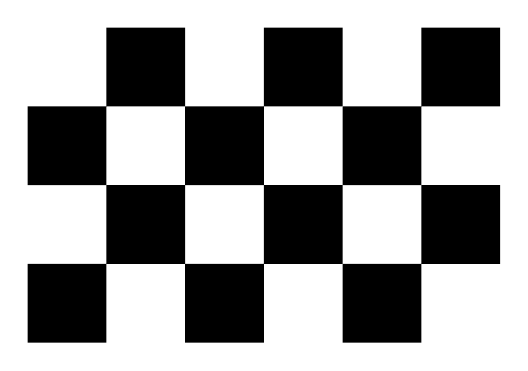
\begin{tikzpicture}[x=1cm]
		\foreach \y in {0,2,...,3}{
			\foreach \x in {0,2,...,4}{
				\fill (\x,\y) rectangle (1+\x,1+\y) rectangle (2+\x,2+\y);}}
	\end{tikzpicture}
\end{center}

Para saber de quantas formas podemos fazer o preenchimento da forma, precisamos numerar as peças pretas e brancas em uma ordem arbitrária.

\begin{center}
	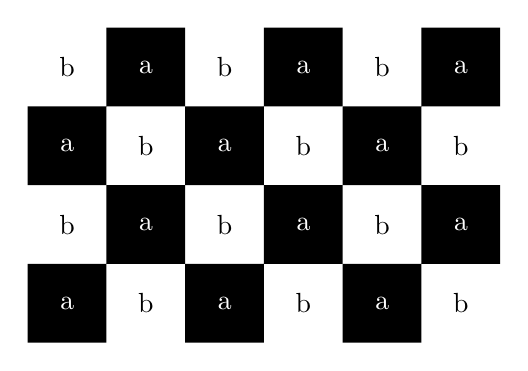
\begin{tikzpicture}[x=1cm]
		\foreach \y in {0,2,...,3}{
			\foreach \x in {0,2,...,4}{
				\draw[black] (1.5+\x, 0.5+\y) node {b};
				\draw[black] (0.5+\x, 1.5+\y) node {b};
				\fill (\x,\y) rectangle (1+\x,1+\y) rectangle (2+\x,2+\y);
				\draw[white] (0.5+\x, 0.5+\y) node {a};
				\draw[white] (1.5+\x, 1.5+\y) node {a};
			}}
	\end{tikzpicture}
\end{center}

Se numerarmos eles e criarmos uma matriz "de adjacência" onde se preenche com $1$ onde dois números são vizinhos horizontais no tabuleiro e $i$ quando são vizinhos verticais. Preenchemos com 0 quando não o são. Teremos nosso resultado calculado quando fizermos o determinante de tal matriz. Isto é, o determinante desta matriz de vizinhança das casas ordenadas dentro das classes nos dá de quantas formas (em módulo e real) podemos preencher o plano com esses dominós.

\subsubsection{O diamante}

O algoritmo que seguiremos é descrito em \cite{propp2002generalized} .Suponha agora o tabuleiro especial:

\begin{center}
	\begin{tikzpicture}[x=1cm]
		\foreach \y in {-5,...,5}{
			\foreach \x in {-5,...,5}{
				\pgfmathparse{abs(\y-0.5) + abs(\x-0.5)}
				\ifnum 5 > \pgfmathresult
					\draw (\x,\y) rectangle (\x,\y) rectangle (1+\x,1+\y);
				\fi
			}
		}
	\end{tikzpicture}
\end{center}

Conseguimos o preencher com os dominós? Podemos seguir o seguinte algoritmo. Suponho o caso mais básico do tabuleiro:

\begin{center}
	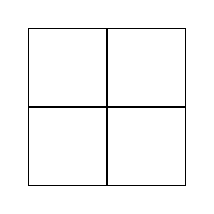
\begin{tikzpicture}[x=1cm]
		\foreach \y in {-5,...,5}{
			\foreach \x in {-5,...,5}{
				\pgfmathparse{abs(\y-0.5) + abs(\x-0.5)}
				\ifnum 2 > \pgfmathresult
				\draw (\x,\y) rectangle (\x,\y) rectangle (1+\x,1+\y);
				\fi
			}
		}
	\end{tikzpicture}
\end{center}

Este podemos fazer o tiling de duas formas triviais,


\begin{center}
	\begin{minipage}[c]{.2\linewidth}
		\centering
		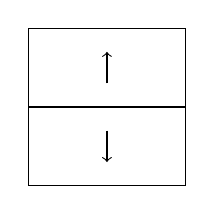
\begin{tikzpicture}[x=1cm]
			\foreach \y in {1,...,2}{
				\draw (0,\y) rectangle (0,\y) rectangle (2,1+\y);
			}
			\draw[->]  (1,2.3) -- (1,2.7);
			\draw[->]  (1,1.7) -- (1,1.3);
		\end{tikzpicture}
	\end{minipage}
	\begin{minipage}[c]{.2\linewidth} %inequalities
		\centering
		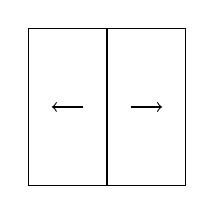
\begin{tikzpicture}[x=1cm]
			\foreach \x in {1,...,2}{
				\draw (\x,0) rectangle (\x,0) rectangle (\x+1,2);
			}
			\draw[->]  (1.7,1) -- (1.3,1);
			\draw[->]  (2.3,1) -- (2.7,1);
		\end{tikzpicture}
	\end{minipage}
\end{center}

Realizaremos o tiling de uma grade expandida utilizando de uma técnica curiosa. Note as setas nos dois dominós que demonstramos. Elas vão indicar a direção de deslocamento que as peças devem tomar quando expandirmos o plano. Ou seja:


\begin{center}
	\begin{minipage}[c]{.4\linewidth}
		\centering
		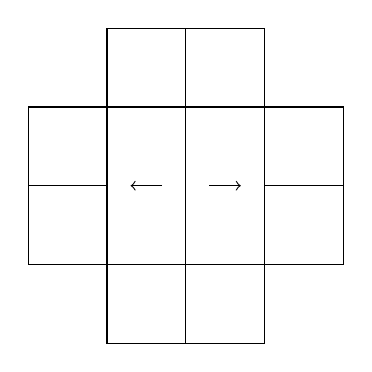
\begin{tikzpicture}[x=1cm]
			\foreach \y in {-5,...,5}{
				\foreach \x in {-5,...,5}{
					\pgfmathparse{abs(\y-0.5) + abs(\x-0.5)}
					\ifnum 3 > \pgfmathresult
					\draw (\x,\y) rectangle (\x,\y) rectangle (1+\x,1+\y);
					\fi
				}
			}
			\foreach \x in {0,...,1}{
				\fill[white] (\x,0) rectangle (\x,0) rectangle (\x+1,2);
				\draw(\x,0) rectangle (\x,0) rectangle (\x+1,2);
			}
			\draw[->]  (0.7,1) -- (0.3,1);
			\draw[->]  (1.3,1) -- (1.7,1);
		\end{tikzpicture}
	\end{minipage}
	\begin{minipage}[c]{.4\linewidth} %inequalities
		\centering
		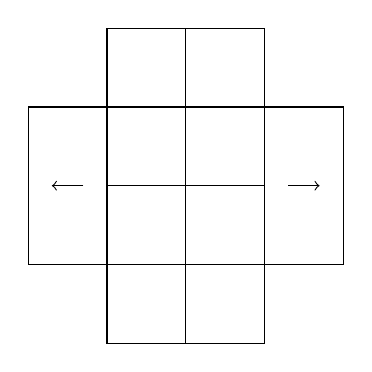
\begin{tikzpicture}[x=1cm]
			\foreach \y in {-5,...,5}{
				\foreach \x in {-5,...,5}{
					\pgfmathparse{abs(\y-0.5) + abs(\x-0.5)}
					\ifnum 3 > \pgfmathresult
					\draw (\x,\y) rectangle (\x,\y) rectangle (1+\x,1+\y);
					\fi
				}
			}
			
			\fill[white] (-1,0) rectangle (-1,0) rectangle (0,2);
			\draw(-1,0) rectangle (-1,0) rectangle (0,2);
			
			\fill[white] (2,0) rectangle (2,0) rectangle (3,2);
			\draw(2,0) rectangle (2,0) rectangle (3,2);
			
			\draw[->]  (-0.3,1) -- (-0.7,1);
			\draw[->]  (2.3,1) -- (2.7,1);
		\end{tikzpicture}
	\end{minipage}
\end{center}


Note que ao final de cada procedimento sempre restará quadrados de $2x2$ completos que podem ser preenchidos independentemente com as duas opções que demos. Às vezes células terão celular que colidem. Devemos eliminar estas e é possível mostrar qus estes vem em pares e são equivalentes quando as peças que colidem são eliminadas. Podemos preencher ambos de volta os fazendo diferentes e vale algo curioso. Para cada malha de $n$-tamanho terão (mesmo que com o artifício descrito) $n$ novos quadrados a se preencher de $2$ maneiras. Ou seja, o tiling final pode ser preenchido de $2^{1+2+3+\cdots+n}$ formas. Escrevendo o modelo em código:

\inputminted[
frame=lines,
framesep=2mm,
baselinestretch=1.2,
bgcolor=white,
fontsize=\footnotesize,
linenos]{FORTRAN}{./code/Tilings.f}

E temos de saída:

\begin{center}
	\includegraphics[scale=0.33]{images/AstecDiamond}
\end{center}










